\chapter{\IfLanguageName{dutch}{Stand van zaken}{State of the Art}}%
\label{ch:stand-van-zaken}

% Tip: Begin elk hoofdstuk met een paragraaf inleiding die beschrijft hoe dit hoofdstuk past binnen het geheel van de bachelorproef. Geef in het bijzonder aan wat de link is met
% het vorige en volgende hoofdstuk.

% Pas na deze inleidende paragraaf komt de eerste sectiehoofding.

% Dit hoofdstuk bevat je literatuurstudie. De inhoud gaat verder op de inleiding, maar zal het onderwerp van de bachelorproef *diepgaand* uitspitten. De bedoeling is dat de lezer na
% lezing van dit hoofdstuk helemaal op de hoogte is van de huidige stand van zaken (state-of-the-art) in het onderzoeksdomein. Iemand die niet vertrouwd is met het onderwerp, weet nu
% voldoende om de rest van het verhaal te kunnen volgen, zonder dat die er nog andere informatie moet over opzoeken \autocite{Pollefliet2011}.

% Je verwijst bij elke bewering die je doet, vakterm die je introduceert, enz.\ naar je bronnen. In \LaTeX{} kan dat met het commando \texttt{$\backslash${textcite\{\}}} of
% \texttt{$\backslash${autocite\{\}}}. Als argument van het commando geef je de ``sleutel'' van een ``record'' in een bibliografische databank in het Bib\LaTeX{}{}-formaat (een
% tekstbestand). Als je expliciet naar de auteur verwijst in de zin (narratieve referentie), gebruik je \texttt{$\backslash${}textcite\{\}}. Soms is de auteursnaam niet expliciet een
% onderdeel van de zin, dan gebruik je \texttt{$\backslash${}autocite\{\}} (referentie tussen haakjes). Dit gebruik je bv.~bij een citaat, of om in het bijschrift van een overgenomen
% afbeelding, broncode, tabel, enz. te verwijzen naar de bron. In de volgende paragraaf een voorbeeld van elk.

% \textcite{Knuth1998} schreef een van de standaardwerken over sorteer- en zoekalgoritmen. Experten zijn het erover eens dat cloud computing een interessante opportuniteit vormen,
% zowel voor gebruikers als voor dienstverleners op vlak van informatietechnologie~\autocite{Creeger2009}.

% Let er ook op: het \texttt{cite}-commando voor de punt, dus binnen de zin. Je verwijst meteen naar een bron in de eerste zin die erop gebaseerd is, dus niet pas op het einde van
% een paragraaf.
% ----------------------------------------------------------------------------------------------------------------------------------------------------------------------------------------------------------------------------------
Dit hoofdstuk licht toe wat een linter is en wat \LaTeX{} en BibLaTeX zijn. Daarnaast wordt er meer verteld over de huidige stand van zaken binnen de wereld van BibLaTeX-linters, het toont aan waarom het gepast is om deze proof of concept uit te werken en de opportuniteiten die zich bieden binnen dit onderwerp. Alsook wordt er een diepere kijk gegeven aan andere linters, hun functionaliteiten en performantie om een beter inzicht te verwerven in aspecten die van belang kunnen zijn voor het uitwerken van een eigen linter.

\section{Wat is een linter?}
Alvorens er uitgelegd wordt waarom het nuttig is om deze proof of concept uit te werken, is het belangrijk om een goed begrip te hebben van wat er effectief gemaakt wordt en wat het nut ervan is. Het doel van deze proof of concept is om een linter te maken. Maar wat is dat juist?

\textcite{Kamunya2023} legt uit dat linten verwijst naar het proces van broncode automatisch controleren op programmatische en stilistische fouten. Dit houdt in dat een linter programmatisch je code scant om te controleren of er problemen zijn die kunnen leiden tot bugs of inconsistenties met de code-stijl en -gezondheid. De linter is hierbij de tool die ervoor gebruikt wordt.

Een linter is een statische analysetool omdat het de broncode of andere gestructureerde data analyseert zonder de code daadwerkelijk uit te voeren \autocite{Moeller2023}. Het voert een \emph{statische} analyse uit, wat betekent dat het de code inspecteert op basis van de geschreven tekst en structuur ervan, zonder rekening te houden met de daadwerkelijke uitvoering van de code.

Een linter is dus een statische analysetool die broncode of andere gestructureerde data kan analyseren.

\section{\LaTeX{}}
\LaTeX{} (uitspraak: LaTech), een uitbreiding op het \TeX{}-typesetting systeem van Donald E. \textcite{Knuth1984}, is bedoeld voor het opmaken van tekst en wiskundige formules. TeX werd ontwikkeld in 1977 met als doel de typografische kwaliteit te verbeteren. De stabiele versie van TeX kwam uit in 1982 en ondersteunt meerdere talen en 8-bit karakters. \LaTeX{} zelf, ontwikkeld door \textcite{Lamport1994} in 1985, voegt een reeks macro's toe om het gebruik van TeX te vereenvoudigen en heeft zich ontwikkeld tot een standaard voor het produceren van wetenschappelijke en wiskundige documentatie \autocite{Oetiker2023}.

\subsection{Werking}
Personen die al ervaring hebben met \LaTeX{} zullen net als \textcite{Oetiker2023} kunnen bevestigen dat \LaTeX{} functioneert door middel van commando's die de logische structuur van een document definiëren (zoals hoofdstukken, secties, en paragrafen) en dat dit anders is dan de typische \acrfull{WYSIWYG} tekstverwerkers zoals Microsoft Office Word, waar de lay-out interactief wordt bepaald tijdens het typen. \LaTeX{} vereist dat de auteur zijn tekst structureert met behulp van vooraf gedefinieerde commando's die de inleiding van het document bepalen.

\subsection{Voordelen}
\begin{enumerate}
    \item Het biedt professionele vormgeving van lay-outs.
    \item Het ondersteunt de zetting van wiskundige formules.
    \item Het moedigt aan tot goed gestructureerd schrijven. Dit resulteert in duidelijk georganiseerde documenten.
    \item Er zijn veel uitbreidingen beschikbaar via packages om functionaliteit zoals PDF-output en betere font-ondersteuning toe te voegen.
\end{enumerate}

\subsection{Nadelen}
\begin{enumerate}
    \item Het instellen van een volledig nieuwe lay-out kan ingewikkeld en tijdrovend zijn.
    \item Niet ideaal voor zeer ongestructureerde documenten.
    \item Leercurve, de \emph{slechte} gewoontes afleren van typische \acrshort{WYSIWYG} programma's vergt enige tijd om aan te wennen.
\end{enumerate}

\subsection{Conclusie}
\LaTeX{} \autocite{Oetiker2023} wordt vooral gewaardeerd in academische en technische kringen waar de precisie van de inhoud en de structuur voorop staan. Eens er een lay-out template bestaat, is het zeer eenvoudig om veel professionele documenten op te maken op eenzelfde manier. De blijvende populariteit is te danken aan de uitbreidbaarheid, consistentie, brede ondersteuning van wiskundige formules, en de mogelijkheid om complexe documenten zoals proefschriften en wetenschappelijke artikelen nauwkeurig op te maken, ook wel typesetten genoemd.

%--- start: BibLaTeX vs BibTeX ---

\section{BibTeX en BibLaTeX}

\subsection{Inleiding}
BibTeX en BibLaTeX zijn hulpmiddelen die worden gebruikt voor het beheren van referenties in \LaTeX{}-documenten. Beide hulpmiddelen hebben verschillende kenmerken en mogelijkheden die inspelen op verschillende behoeften van gebruikers bij het beheren van bibliografieën. Deze vergelijking belicht de technische aspecten van beide en biedt een diepgaande analyse om de verschillen tussen beide beter te begrijpen.

\subsection{Overzicht van BibTeX}
BibTeX werd in 1985 gecreëerd door \textcite{Patashnik1988} en is ontworpen om samen te werken met \LaTeX{}. Het vergemakkelijkt het genereren van bibliografieën door gebruikers in staat te stellen citatievermeldingen te definiëren in een \texttt{.bib}-bestand en deze te formatteren volgens vooraf gedefinieerde stijlen.

\subsubsection{Belangrijkste Kenmerken van BibTeX}
\begin{enumerate}
    \item \textbf{Compatibiliteit}: BibTeX is compatibel met \LaTeX{} versie 2.09 en latere versies. Het integreert goed met \LaTeX{}-documenten en maakt gebruik van \texttt{.bst}-bestanden voor stijldefinities \autocite{Patashnik1988}.
    \item \textbf{Kruisverwijzingen}: BibTeX ondersteunt kruisverwijzingen (Engels: cross-referencing) tussen vermeldingen, waardoor een vermelding velden van een andere kan erven. Dit is nuttig voor het citeren van proceedings en verzamelwerken \autocite{Patashnik1988}.
    \item \textbf{Geaccentueerde Karakters}: BibTeX kan geaccentueerde karakters verwerken, wat cruciaal is voor internationalisatie. Het vereist dat geaccentueerde karakters tussen accolades worden geplaatst om correcte verwerking te garanderen \autocite{Patashnik1988}.
    \item \textbf{Sorteren en Labels}: BibTeX sorteert vermeldingen standaard op auteur, jaar en titel. Aangepaste sorteer- en labelgeneratie kan worden gespecificeerd in \texttt{.bst}-bestanden \autocite{Patashnik1988}.
    \item \textbf{String-concatenatie}: BibTeX ondersteunt string-concatenatie in veldwaarden, wat de flexibiliteit van vermeldingsdefinities vergroot \autocite{Patashnik1988}.
    \item \textbf{Preambule-commando}: Het \texttt{@PREAMBLE}-commando stelt gebruikers in staat om \LaTeX{}-commando's in de bibliografie op te nemen, wat extra aanpassingsopties biedt \autocite{Patashnik1988}.
\end{enumerate}

\subsubsection{Beperkingen van BibTeX}
\begin{enumerate}
    \item \textbf{Aanpassingsbeperkingen}: Het aanpassen van bibliografische stijlen in BibTeX vereist het maken of wijzigen van \texttt{.bst}-bestanden, die een gespecialiseerde taal bevatten die complex kan zijn voor nieuwe gebruikers \autocite{Patashnik1988}.
    \item \textbf{Unicode Ondersteuning}: BibTeX heeft beperkte ondersteuning voor Unicode, wat een beperking kan zijn voor documenten die uitgebreid gebruik maken van niet-ASCII-karakters \autocite{Patashnik1988}.
    \item \textbf{Statisch Sorteren en Formatteren}: Wijzigingen in sorteren en formatteren vereisen aanpassingen aan de \texttt{.bst}-bestanden, wat niet eenvoudig is voor dynamische of complexe sorteerbehoeften \autocite{Patashnik1988}.
\end{enumerate}

\subsection{Overzicht van BibLaTeX}
BibLaTeX, oorspronkelijk ontwikkeld door Philipp Lehman en later verder door \textcite{Kime2024}, is een moderner en flexibeler alternatief voor BibTeX. Het is ontworpen om samen te werken met de \texttt{biber}-backend en biedt uitgebreide aanpassingsmogelijkheden en geavanceerde functies voor bibliografiebeheer.

\subsubsection{Belangrijkste Kenmerken van BibLaTeX}
\begin{enumerate}
    \item \textbf{Verbeterde Aanpassing}: BibLaTeX maakt uitgebreide aanpassing van bibliografieën mogelijk via \LaTeX{}-macro's. Gebruikers kunnen aangepaste stijlen en citatiecommando's definiëren zonder een aparte programmeertaal te moeten leren \autocite{Kime2024}.
    \item \textbf{Unicode Ondersteuning}: BibLaTeX ondersteunt volledig Unicode, waardoor het geschikt is voor documenten die een breed scala aan karakters en scripts bevatten \autocite{Kime2024}.
    \item \textbf{Dynamisch Sorteren en Filteren}: BibLaTeX biedt krachtige sorteer- en filteropties, waardoor gebruikers vermeldingen dynamisch kunnen sorteren en groeperen op basis van verschillende criteria zoals auteur, jaar en type \autocite{Kime2024}.
    \item \textbf{Meertalige Ondersteuning}: BibLaTeX kan samenwerken met \texttt{babel}- en \texttt{polyglossia}-pakketten om meertalige documenten te ondersteunen. Het past automatisch bibliografie- en citatiestijlen aan op basis van de taalinstellingen van het document \autocite{Kime2024}.
    \item \textbf{Gesegmenteerde Bibliografieën}: Gebruikers kunnen gesegmenteerde bibliografieën en meerdere bibliografieën binnen een enkel document maken, gecategoriseerd op onderwerpen of secties \autocite{Kime2024}.
    \item \textbf{Aanpassing van het Datamodel}: Het datamodel in BibLaTeX kan worden uitgebreid en aangepast, waardoor gebruikers nieuwe vermeldingssoorten en velden kunnen definiëren indien nodig \autocite{Kime2024}.
    \item \textbf{Annotatie en Annotatiecommando's}: BibLaTeX ondersteunt data-annotatie en querycommando's, waardoor meer geavanceerd beheer van bibliografische gegevens mogelijk is \autocite{Kime2024}.
\end{enumerate}

\subsubsection{Beperkingen van BibLaTeX}
\begin{enumerate}
    \item \textbf{Leercurve}: De uitgebreide aanpassingsmogelijkheden en flexibiliteit van BibLaTeX brengen een steilere leercurve met zich mee in vergelijking met BibTeX \autocite{Kime2024}.
    \item \textbf{Compatibiliteitsproblemen}: BibLaTeX is niet volledig compatibel met sommige oudere \LaTeX{}-pakketten die specifiek voor BibTeX zijn ontworpen. Gebruikers moeten ervoor zorgen dat hun documentopstelling compatibel is met BibLaTeX \autocite{Kime2024}.
    \item \textbf{Afhankelijkheid van Biber}: BibLaTeX is afhankelijk van de \texttt{biber}-backend voor het verwerken van bibliografiebestanden, wat een extra afhankelijkheid met zich meebrengt en installatie- en configuratie-inspanningen kan vereisen \autocite{Kime2024}.
\end{enumerate}

\subsection{Gedetailleerde Vergelijking}

\subsubsection{Database-vermeldingssoorten}
BibTeX en BibLaTeX ondersteunen verschillende soorten vermeldingen voor verschillende soorten referenties. BibLaTeX biedt echter meer flexibiliteit en extra vermeldingssoorten die niet beschikbaar zijn in BibTeX.

\begin{itemize}
    \item \textbf{BibTeX}: Standaard vermeldingssoorten zijn onder andere \texttt{article}, \texttt{book}, \texttt{inbook}, \texttt{incollection}, \texttt{inproceedings}, \texttt{manual}, \texttt{mastersthesis}, \texttt{misc}, \texttt{phdthesis}, \texttt{proceedings}, \texttt{techreport}, en \texttt{unpublished} \autocite{Patashnik1988}.
    \item \textbf{BibLaTeX}: Ondersteunt alle BibTeX-vermeldingssoorten en extra zoals \texttt{mvbook} (meerdelige boeken), \texttt{mvcollection} (meerdelige verzamelingen), \texttt{dataset}, \texttt{online}, \texttt{patent}, en meer. Elke vermeldingssoort kan een rijk stel velden hebben die zijn afgestemd op specifieke referentiebehoeften \autocite{Kime2024}.
\end{itemize}

\subsubsection{Citatie- en Bibliografiecommando's}
BibLaTeX biedt een breed scala aan citatiecommando's en bibliografiebeheeropties die de mogelijkheden van BibTeX overtreffen.

\begin{itemize}
    \item \textbf{BibTeX}: Basis citatiecommando's zijn \texttt{\textbackslash cite}, \texttt{\textbackslash nocite}, \texttt{\textbackslash bibliography}, en \texttt{\textbackslash bibliographystyle} \autocite{Patashnik1988}.
    \item \textbf{BibLaTeX}: Biedt uitgebreide citatiecommando's zoals \texttt{\textbackslash cite}, \texttt{\textbackslash parencite}, \texttt{\textbackslash footcite}, \texttt{\textbackslash textcite}, en meer. Bibliografiecommando's bieden fijnere controle over het sorteren, filteren en formatteren van vermeldingen \autocite{Kime2024}.
\end{itemize}

\subsubsection{Aanpassing en Stijldefinitie}
BibTeX en BibLaTeX verschillen aanzienlijk in hun benadering van aanpassing en stijldefinitie.

\begin{itemize}
    \item \textbf{BibTeX}: Aanpassing vereist het wijzigen van \texttt{.bst}-bestanden, wat een gespecialiseerde en minder intuïtieve taal inhoudt \autocite{Patashnik1988}.
    \item \textbf{BibLaTeX}: Aanpassing gebeurt met behulp van \LaTeX{}-macro's, waardoor het toegankelijker is voor gebruikers die bekend zijn met \LaTeX{}. Gebruikers kunnen eenvoudig citatie- en bibliografiestijlen definiëren en aanpassen binnen hun \LaTeX{}-documenten \autocite{Kime2024}.
\end{itemize}

\subsubsection{Compatibiliteit en Integratie}
BibTeX is meer gevestigd en heeft daarom een bredere compatibiliteit met oudere \LaTeX{}-pakketten, terwijl BibLaTeX moderne functies biedt maar compatibiliteitsproblemen kan ondervinden met sommige oudere pakketten.

\begin{itemize}
    \item \textbf{BibTeX}: Compatibel met de meeste oudere \LaTeX{}-pakketten en stijlen \autocite{Patashnik1988}.
    \item \textbf{BibLaTeX}: Vereist specifieke versies van \LaTeX{} en \texttt{biber}, en is mogelijk niet compatibel met alle pakketten die voor BibTeX zijn ontworpen \autocite{Kime2024}.
\end{itemize}

\subsection{Conclusie}
Zowel BibTeX als BibLaTeX spelen een belangrijke rol in het beheer van bibliografieën binnen \LaTeX{}-documenten. BibTeX is geschikt voor gebruikers die een eenvoudige, gevestigde oplossing nodig hebben met brede compatibiliteit. BibLaTeX daarentegen is ideaal voor degenen die geavanceerde functies, uitgebreide aanpassing en moderne mogelijkheden zoals Unicode-ondersteuning en dynamisch bibliografiebeheer nodig hebben. Gebruikers moeten het hulpmiddel kiezen dat het beste aansluit bij hun technische vereisten en document specificaties. Bij HOGENT is het gebruik van BibLaTeX verplicht. Deze proof of concept is daarom bijzonder relevant, aangezien het kan bijdragen aan het voldoen aan de behoeften van zowel studenten als docenten door te zorgen dat de gebruikte BibLaTeX-bestanden optimaal georganiseerd en correct zijn.

%--- end: BibLaTeX vs BibTeX ---
\section{Huidige stand van zaken}
Op het ogenblik van het schrijven zijn er nog geen \emph{optimale} BibLaTeX-Linters beschikbaar en de linters van de voorganger BibTeX zijn niet compatibel met BibLaTeX. De enige beschikbare linter voor BibLaTeX op dit moment staat op een GitHub-repository van Pez Cuckow\footnote{\label{foot:pezgithub}\url{https://github.com/Pezmc/BibLaTeX-Linter}}. Deze hoort functioneel te zijn, maar lijkt niet optimaal wat de code betreft. Er is dus duidelijk mogelijkheid tot verbetering. De BibLaTeX-Linter van Pez Cuckow is geschreven in Python en heeft een webinterface. Naast het feit dat deze lastig werkend te krijgen was, werkt deze ook zeker niet zonder fouten. Het is mogelijk om deze effectief uit te testen, maar bij het testen werd er gemerkt dat er fouten optraden die niet direct op te lossen waren, zie Figuur~\ref{fig:biblatex-linter-error}. Het was niet mogelijk om zomaar elk .bib-bestand te gebruiken bij deze checker, wat het niet gunstig maakt om te gebruiken. Wel was het interessant om te kijken hoe Cuckow bepaalde aspecten interpreteerde en uitvoerde. Dit was uiteindelijk ook een bron waaruit inspiratie gehaald kon worden.

\begin{figure}[ht]
    \centering
    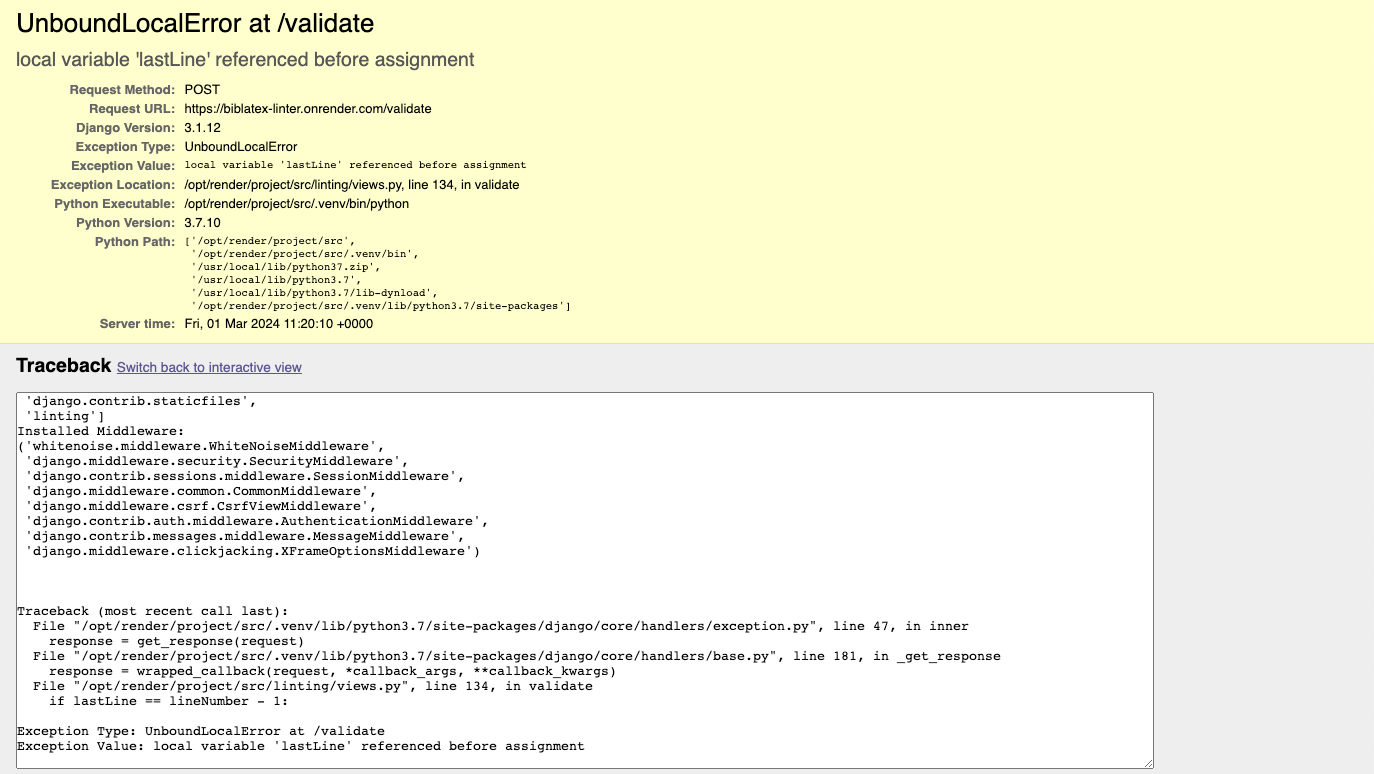
\includegraphics[width=0.7\textwidth]{./files/Pezmc-LinterError_cropped.png}
    \caption[Foutmelding BibLaTeX-linter]{Lintingerror bij het valideren van een BibLaTeX-bestand, gebruikmakende van de linter geschreven door Pez Cuckow\footnote[1]{\ref{foot:pezgithub}}.}
    \label{fig:biblatex-linter-error}
\end{figure}

Daarnaast leek de aanpak van de geschreven code ook niet optimaal te zijn op vlak van leesbaarheid en uitbreidbaarheid. Gezien dit echter wel criteria zijn waaraan de proof of concept moest voldoen, werd er besloten om deze linter niet verder te onderzoeken. Er werd wel gekeken naar de functionaliteiten die deze linter aanbood en andere zaken die handig leken om over te nemen in de eigen implementatie.

\section{Andere linters}
Gezien het wat BibLaTeX-linters betreft zeer beperkt is, werd er op zoek gegaan naar andere soorten linters. Bijvoorbeeld een linter voor JavaScript, Python of andere programmeertalen. Er werd gekeken naar het soort features dat de linters aanbieden, hun performantie, alsook hun broncode indien deze toegankelijk was. Enkele linters die bekeken werden zijn: JSHint, Stylelint, Ruff, PyType en bibl. Net als de proof of concept waren al de bekeken linters gratis te gebruiken en open source.

Daaruit bleek dat naast de manier van implementeren, de taal waaruit de linter opgebouwd is ook van belang is voor de performantie. Dit was het begin naar een onderzoek voor de ideale programmeertaal te vinden voor deze proof of concept.

\subsection{Ruff}
Ruff\footnote{\url{https://astral.sh/ruff}} is een Python linter ontwikkeld door \textcite{Astral2024}, geschreven in de programmeertaal Rust. Dit onderscheidt Ruff van andere Python linters, die doorgaans in Python zelf zijn geschreven. Rust staat bekend om zijn snelheid en veiligheid, wat het een uitstekende keuze maakt voor een linter. Bovendien is Rust lichter om op hardware te draaien dan Python, aangezien Python een interpretatieve taal is en Rust een gecompileerde taal. Dit maakt Ruff bijzonder geschikt voor gebruik in CI-pipelines.

Een ander belangrijk voordeel van Rust is de stabiliteit van de taal. Er is slechts één versie van Rust en die wordt continu doorontwikkeld, wat ervoor zorgt dat code die vandaag gecompileerd wordt, ook over tien jaar nog gecompileerd kan worden. Dit biedt een aanzienlijke zekerheid voor de toekomstbestendigheid van software.

Ruff kan op bepaalde taken tien tot wel honderd keer sneller zijn dan zijn concurrenten. Dit wekt vanzelfsprekend de interesse om de prestaties van de Rust-taal te testen. Op de website van Astral, de makers van Ruff, is een vergelijking te vinden tussen Ruff en andere Python linters. Ook \textcite{TurnerTrauring2023} bevestigen in hun artikel dat de snelheid van Ruff duidelijk merkbaar is en onderbouwen dit met testresultaten. Deze prestaties zijn vooral voordelig in pipelines op virtuele machines, aangezien vCPU's (virtuele processor units) meestal trager zijn dan de verwerkingsunits in moderne laptops of desktops.

\subsection{DirtyRat}
\label{subsec:dirtyrat}
DirtyRat is een JavaScript linter die werd ontdekt tijdens het onderzoek naar hoe een linter gemaakt kon worden. Het is een linter die zelf in JavaScript geschreven is en waarvan de stapsgewijze opbouw te vinden is in het artikel van \textcite{BorgesLate2021}. Daarnaast is ook de broncode zelf te vinden op GitHub\footnote{\url{https://github.com/JoanaBLate/dirtyrat}}. Dit was ook de reden waarom er besloten werd om JavaScript als kandidaat-programmeertaal te nemen.

Hoewel het artikel zeer in detail gaat en het grondig onderzocht werd, werd er vastgesteld dat het toch wat te uitgebreid is voor deze proof of concept. JavaScript en andere programmeertalen hebben veel meer complexe structuren dan een BibLaTeX-bestand. Dus hoewel het interessant was om te zien hoe een linter in JavaScript gemaakt kon worden, was het niet nodig om elke component over te nemen.

\subsection{bibl}
bibl\footnote{\url{https://gitlab.com/arnevdk/bibl}} is een linter voor BibTeX, de voorloper van BibLaTeX, geschreven in Python door Arne Van Den Kerchove. Het onderzoeken van een linter voor de voorloper van BibLaTeX leek bijzonder interessant om een goed inzicht te krijgen in wat precies verwacht kan worden van een linter. bibl biedt een uitgebreide lijst van regels, evenals een gedetailleerde projectstructuur en implementatiewijze van zowel de lintercode als de bijbehorende tests.

bibl werd ontdekt net voordat er begonnen werd met de ontwikkeling van een eigen linter. Na een grondige analyse bleek dat bibl een goed opgebouwde, modulaire en efficiënte open-source linter is. bibl voldeed aan vrijwel alle criteria die voor de proof of concept linter waren opgesteld, wat leidde tot een nieuwe visie.

Het maken van een linter zoals bibl, maar dan voor BibLaTeX in plaats van BibTeX, leek een haalbaar einddoel. Echter, vanwege een achterstand op de planning, zou het niet mogelijk zijn om een eigen linter even uitgebreid uit te werken. Hoewel het concept van een proof of concept wellicht bereikt kon worden, leek het voordeliger om bibl te proberen gebruiken en compatibel te maken met BibLaTeX.

Gezien de verschillen tussen BibTeX en BibLaTeX, was er enige twijfel over de haalbaarheid hiervan, vooral omdat bibl gebruik maakt van pybtex als parser. Op de site van pybtex\footnote{\url{https://pybtex.org/}} staat het volgende vermeld:

\begin{quote}\emph{Pybtex is a BibTeX-compatible bibliography processor written in Python.}\end{quote}

Dit impliceert dat pybtex verantwoordelijk is voor het extraheren van gegevens uit bibliografiebestanden. Hoewel de quote niet expliciet vermeldt dat het alleen voor BibTeX-bestanden werkt, wordt compatibiliteit met BibLaTeX nergens expliciet genoemd. Daarom was het noodzakelijk om dit zelf te testen.

Voor de test werd een BibLaTeX-document gebruikt dat door de promotor was gedeeld. Dit document bevatte geldige bronvermeldingen en was daarmee perfect geschikt om te onderzoeken of bibl als basis gebruikt kon worden. bibl werd snel geïnstalleerd via de Python package manager, pip. Vervolgens werd het lint-commando uitgevoerd op het BibLaTeX-document en werd bekeken wat bibl rapporteerde.

bibl crashte niet en genereerde een uitgebreide lijst opmerkingen; dit was een positief resultaat. Er waren echter enkele bestaande regels die niet compatibel waren met BibLaTeX-bestanden.

\subsubsection{Algemene structuur}
\begin{figure}[ht]
    \centering
    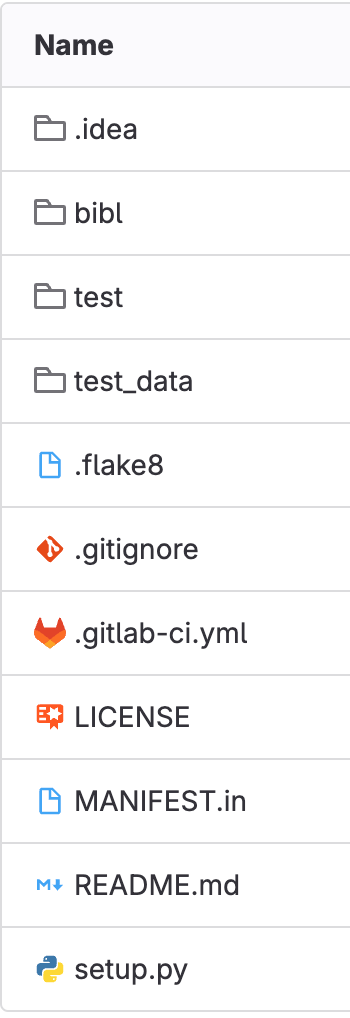
\includegraphics[width=0.3\textwidth]{./files/bibl_repo.png}
    \caption[bibl repository]{Repository overzicht bibl.}
    \label{fig:bibl_repo}
\end{figure}

De gitlab-repository van bibl\footnote{\url{https://gitlab.com/arnevdk/bibl}} is een goed voorbeeld van hoe een goed gestructureerd project eruit kan zien. Naast de bibl folder, die alle broncode van bibl zelf bevat, zijn er ook: testen, test-data, lintervoorkeuren, een pipeline (zie \ref{sec:pipelines}), een licentie, een duidelijke readme en een installatie-script aanwezig. Ook de .idea, .gitignore en MANIFEST.in zijn niet onbelangrijk. de .idea bevat de voorkeursinstellingen voor de IDE (Integrated development environment, ook gekend als werkomgeving) van de auteur, het .gitignore bestand bevat een opsomming van bestanden of soort bestanden die niet op de repository dienen te komen. Denk hier aan tijdelijke bestanden die vanzelf aangemaakt worden; deze zijn niet nodig op de repository omdat ze onnodig plaats gebruiken. Tot slot wordt het MANIFEST.in bestand in Python gebruikt om aan te geven welke bestanden moeten worden opgenomen bij het maken van een distributiepakket; wat nodig is om het beschikbaar te stellen bij de pakketbeheerder\footnote{\url{https://pypi.org/}} (pip). In een latere sectie (\ref{sec:bibl-in-depth}) wordt er dieper ingegaan op de volledige werking van de linter.
% ---
\section{Programmeertaal}

Om de gepaste programmeertaal te vinden, werden diverse kandidaat\babelhyphen{hard}programmeertalen overwogen. De kandidaat\babelhyphen{hard}programmeertalen waren: Rust, JavaScript en Python. Door het analyseren van reeds bestaande linters en het afgaan van een hele lijst aan programmeertalen, werd er besloten om met deze drie programmeertalen te experimenteren.

In een latere fase (sectie \ref{sec:mini-pocs}) werden er beperkte prototypes uitgewerkt in elk van deze talen; deze werden met elkaar vergeleken om te bepalen welke taal het meest geschikt zou zijn. Alle opties zijn cross-platform, wat belangrijk is gezien de linter bruikbaar dient te zijn voor iedereen. Alsook dient het een programmeertaal te zijn die gekend is, hiermee wordt er bedoeld dat het een programmeertaal moet zijn die al matuur is en door een groot aantal mensen gekend is.

\subsection{Rust}
Gezien de performantie van Ruff, leek Rust een gepaste optie om de linter in te maken. Ook de stijgende populariteit van de taal maakt dit een aantrekkelijke optie. Ondanks dat dit een onbekende taal is, leek het zeker wel een interessante taal om te leren. De haalbaarheid van de proof of concept kwam echter meer in gevaar door deze keuze. Hoewel de populariteit stijgt, blijft het wel nog een taal die niet door iedereen gekend is, in tegenstelling tot bijvoorbeeld JavaScript of Python. Een ander groot pluspunt aan Rust is dat code die vandaag compiled, ook nog binnen vijf of tien jaar zal kunnen compilen. Dit omdat de makers ervoor streven dat het een super compatibele programmeertaal is. Wat men niet met volle zekerheid van bijvoorbeeld Python\footnote{\url{https://devguide.python.org/versions/}} zou kunnen zeggen.

Dankzij \textcite{Klabnik2022} kan er geleerd worden dat Rust een nadruk legt op typeveiligheid (typesafety) en geheugenveiligheid. Wanneer een taal of systeem geheugenveilig is, betekent dit dat het ontworpen is om toegangsfouten zoals bufferoverlopen, dangling pointers (verwijzingen naar vrijgegeven geheugen), en dubbele bevrijdingen van geheugen (double frees) te voorkomen. Deze soorten fouten kunnen leiden tot onvoorspelbaar gedrag, crashes, en beveiligingslekken zoals het uitvoeren van willekeurige code of informatie-lekken. Het is daarom een goede eigenschap om te hebben.

\subsection{Python}
Python was wellicht stukken trager in vergelijking met Rust in de test die gevonden werd, maar het blijft wel een taal waar iedereen gemakkelijk mee kan beginnen te werken. Voor het gemak van uitbreidbaarheid is dit dan weer een interessante optie om deze taal in optie te nemen. Zoals eerder vermeld door \textcite{TurnerTrauring2023} zou de performantie vooral bij de pipeline te merken zijn.
De echte vraag blijft momenteel nog altijd in hoeverre het minder performant zijn een grote zorg zal worden voor deze proof of concept.

\subsection{JavaScript}
Een zeer gekende scripting taal dat cross-platform gebruikt kan worden. Hoewel het eerder gericht is voor het gebruik in websites of \acrshort{GUI} gerichte scripts, is het ook mogelijk om er cli-tools mee te maken. De performantie werd onderzocht. JavaScript is ook een dynamisch typerende taal, wat in theorie voor problemen zou kunnen zorgen in sommige use-cases, al leek dit geen zorg te zijn voor deze proof of concept\autocite{Simpson2023}.

\section{Opbouw linter}
Aan het begin van dit project werd de beslissing genomen om direct met de ontwikkeling van een prototype aan de slag te gaan, wat leidde tot de zoektocht naar geschikte bronnen. Deze beslissing werd genomen gezien de beperkte tijd en de hoeveelheid aan onderzoek die diende te gebeuren. Indien Rust de taal zou moeten worden, moest deze nog volledig aangeleerd worden en zou er immers geen kostbare tijd verloren mogen gaan.

In dit proces werden de artikelen van \textcite{BorgesLate2021}, die een stapsgewijze handleiding bieden voor het bouwen van een JavaScript-linter, als bijzonder nuttig beschouwd. Ondanks dat de lectuur van deze serie aanvankelijk de indruk wekte dat het project complexer zou zijn dan verwacht, veranderde dit vermoeden na verder onderzoek naar de structuur van .bib-bestanden. Het werd duidelijk dat de ontwikkeling van een linter voor BibLaTeX minder complex is dan voor programmeertalen. Dit is te wijten aan het feit dat programmeertalen loops, conditionele statements en een scala aan andere complexe elementen bevatten, terwijl BibLaTeX gekenmerkt wordt door een consistente en gestandaardiseerde structuur, waardoor de noodzaak voor het opleggen van regels aanzienlijk vermindert. Het was echter wel zeer nuttig om alle componenten te zien die aan bod kunnen komen bij het bouwen van een linter en om deze in gedachte te houden voor de effectieve uitwerking van de BibLaTeX-linter proof of concept.

\section{bibl pakket - diepere blik}
\label{sec:bibl-in-depth}
\begin{figure}[ht]
    \centering
    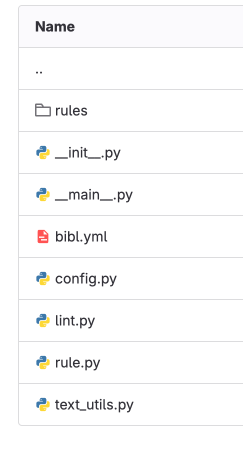
\includegraphics[width=0.4\textwidth]{./files/bibl_src.png}
    \caption[bibl repository - Source code]{Repository overzicht bibl broncode.}
    \label{fig:bibl_src}
\end{figure}

De structuur van bibl \ref{fig:bibl_src} volgt een gebruikelijke pakket-gebaseerde aanpak voor het organiseren van code. Deze aanpak wordt vaak toegepast wanneer een project is opgezet als een herbruikbaar pakket, in plaats van een los script. De aanwezigheid van \texttt{\_\_init\_\_.py} zorgt er namelijk voor dat het pakket importeerbaar is \autocite{Loubser2021}. Dit is direct ook een indicator dat het om een pakket gaat.

Om bibl te begrijpen, wordt de broncode van bibl zelf geanalyseerd. Gezien \texttt{bibl} uiteindelijk de basis kon worden van deze proof of concept, was het van groot belang om een zorgvuldige analyse uit te voeren en de codebase zo goed mogelijk te begrijpen.

\subsection{\_\_init\_\_.py}
Zoals eerder vermeld, is dit bestand kenmerkend bij pakketten. Het bestand is namelijk vereist voor Python om de directory als een pakket te behandelen. Het kan leeg zijn, maar het kan ook initialisatiecode of pakket-niveau-definities bevatten; in dit geval bevat het de huidige softwareversie.

\subsection{\_\_main\_\_.py}
Dit bestand wordt gebruikt wanneer het pakket als een script wordt uitgevoerd (bijvoorbeeld \texttt{python -m bibl}). Het bevat de implementatie van de \acrfull{CLI} voor het linten van bibliografische bestanden in BibTeX-formaat. Het script, hiervoor als referentie bestand, maakt gebruik van de \texttt{Click}-bibliotheek om een gebruiksvriendelijke interface te bieden voor het controleren van bibliografische referenties op consistentie en correctheid. Hieronder volgt een overzicht van de verschillende onderdelen binnen dit bestand.

\subsubsection{Imports en Configuratie}

Het script begint met het importeren van noodzakelijke modules en functies, waaronder \texttt{Click} voor het \acrshort{CLI}-framework, en functies uit de \texttt{bibl}-module voor linting, configuratie en regels:

\begin{minted}[autogobble, breaklines, linenos, samepage]{python3}
import os
import warnings
import click
from bibl import __version__
from bibl.lint import lint as bibl_lint
from bibl.config import load_config_file, set_config
from bibl.rule import load_rules
from bibl.text_utils import format_rules_markdown_tables
\end{minted}
\captionof{listing}[bibl: \_\_main\_\_.py - Imports ]{bibl: \_\_main\_\_.py - Imports. \label{lst:bibl_main_imports}}

\subsubsection{\acrshort{CLI} Basisgroep}

Een \acrshort{CLI} basisgroep functioneert als een container, of groepering, voor meerdere gerelateerde command-line commando's. Hiermee wordt het mogelijk gemaakt om een hoofdcommando te definiëren waaraan subcommando's kunnen worden toegevoegd.
De basisgroep wordt gedefinieerd met behulp van de \texttt{@click.group()} decorator. Deze groep fungeert als een container voor subcommando's die specifieke taken uitvoeren. De subcommando's kunnen tegelijkertijd ook als parameter beschouwd worden. Opties die van toepassing zijn op de gehele groep kunnen hier ook worden gespecificeerd. Een voorbeeld van de definitie van een basisgroep in het script is als volgt:

\begin{minted}[autogobble, breaklines, linenos]{python3}
@click.group()
@click.option('-c', '--config', help='Custom configuration file path.', type=str)
@click.option('--select', help='Comma separated list of enabled rules, all other rules will be disabled.', type=str)
@click.option('--ignore', help='Comma separated list of disabled rules, all other rules will be enabled.', type=str)
@click.option('--indent-spaces', help='Number of trailing whitespaces for indented line, used by TO1.', type=int)
@click.option('--max-line-length', help='Max line length before wrap recommended, used by T03.', type=int)
def cli(config, select, ignore, indent_spaces, max_line_length):
    if config is not None:
        load_config_file(config)
    elif os.path.isfile('bibl.yml'):
        load_config_file('bibl.yml')
    elif os.path.isfile('.bibl.yml'):
        load_config_file('.bibl.yml')
    if select is not None:
        set_config('select', select.split(','))
    if ignore is not None:
        set_config('ignore', ignore.split(','))
    set_config('indent_spaces', indent_spaces)
    set_config('max_line_length', max_line_length)
\end{minted}
\captionof{listing}[bibl: \_\_main\_\_.py - \acrshort{CLI} parameters ]{bibl: \_\_main\_\_.py - \acrshort{CLI} parameters. \label{lst:bibl_main_cli}}

\subsubsection{Lint Commando}

Het \texttt{lint} commando lint één of meer opgegeven BibTeX-bestanden:

\begin{minted}[autogobble, breaklines, linenos, samepage]{python3}
@cli.command(help="Lint a BibTeX bibliography file.")
@click.argument('bibliography', type=str, nargs=-1)
def lint(bibliography):
    warnings.filterwarnings("ignore")
    for bib in bibliography:
        bibl_lint(bib)
\end{minted}
\captionof{listing}[bibl: \_\_main\_\_.py - Commando: lint ]{bibl: \_\_main\_\_.py - Lint commando. \label{lst:bibl_main_lint_command}}

\subsubsection{Lijst Commando's}

Er zijn twee commando's om de lintingregels weer te geven: \texttt{list\_all} toont alle beschikbare regels, terwijl \texttt{list\_enabled} alleen de ingeschakelde regels toont.

\begin{minted}[autogobble, breaklines, linenos]{python3}
@cli.command(help="Show all available rules.")
@click.option('-m', 'markdown', help='Format rules as markdown table.', is_flag=True)
def list_all(markdown):
    rules = load_rules().all
    if markdown:
        click.echo(format_rules_markdown_tables(rules))
    else:
        for rule in rules:
            click.echo(rule)

@cli.command(help="Show all rules enabled by the configuration.")
@click.option('-m', 'markdown', help='Format rules as markdown table.', is_flag=True)
def list_enabled(markdown):
    rules = load_rules().enabled
    if markdown:
        click.echo(format_rules_markdown_tables(rules))
    else:
        for rule in rules:
            click.echo(rule)
\end{minted}
\captionof{listing}[bibl: \_\_main\_\_.py - Commando: toon alle regels]{bibl: \_\_main\_\_.py - Commando om alle regels te tonen. \label{lst:bibl_main_lint_command}}

\subsubsection{Versie Commando}

Het \texttt{version} commando toont de huidige versie van het \texttt{bibl}-pakket:

\begin{minted}[autogobble, breaklines, linenos, samepage]{python3}
@cli.command(help="Show the package version.")
def version():
    click.echo('bibl version: ' + __version__)
\end{minted}
\captionof{listing}[bibl: \_\_main\_\_.py - Commando: huidige versie]{bibl: \_\_main\_\_.py - Toon de huidige versie van het pakket. \label{lst:bibl_version_command}}
\subsubsection{Hoofdprogramma}

Het hoofdprogramma start de \acrshort{CLI} met \texttt{cli(prog\_name='bibl')}:

\begin{minted}[autogobble, breaklines, linenos, samepage]{python3}
if __name__ == '__main__':
    cli(prog_name='bibl')
\end{minted}
\captionof{listing}[bibl: \_\_main\_\_.py - Commando: bibl vanuit \acrshort{CLI}]{bibl: \_\_main\_\_.py - Vanuit \acrshort{CLI} kan bibl rechtstreeks aangeroepen worden. \label{lst:bibl_cli_command}}
%---
\subsection{bibl.yml - Configuratiebestand}
Het volgende configuratiebestand is een YAML (.yml) bestand dat de standaardinstellingen voor de bibliografische lintingtool definieert. Dit bestand specificeert welke regels ingeschakeld of uitgeschakeld moeten worden, evenals andere configuratie-opties zoals de maximale regellengte en het aantal inspringende spaties.

\begin{minted}[autogobble, breaklines, linenos]{yaml}
## DEFAULT BIBL CONFIG
select: [ ] # List of enabled rules, all other rules will be disabled
ignore: [ ] # List of disabled rules, all other rules will be enabled
# Specify max 1 of the two options above. If none are specified, all rules will be enabled
indent_spaces: 4 # number of trailing whitespaces for indented line, used by TO1
max_line_length: 120  # max line length before wrap recommended, used by T03
abbreviation_dot: True  # abbreviate middle names with dot (John F. Kennedy) as opposed to without (John F Kennedy), used by E02

# Specification from https://en.wikipedia.org/wiki/BibTeX extended with fields used in JabRef.
# This specification is used to generate M01 and U01 rules
type_spec:
  article: # An article from a journal or magazine.
    required: [ title, journal, year, volume ]
    optional: [ number, pages, month, doi, key, file ]
  book: # A book with an explicit publisher.
    required: [ title, publisher, year ]
    optional: [ volume, number, series, address, edition, month, key, url, file, isbn ]
# NOTE: Overige entry types weggelaten wegens plaats!
\end{minted}
\captionof{listing}[bibl: bibl.yml - Configuratie]{bibl: bibl.yml - Deel code uit het hoofdconfiguratiebestand. Geselecteerde en te negeren regels kunnen hier toegekend worden. Alsook de standaard aantal spaties ter indentatie. Ook kan er gekozen worden of middelnamen afgekort mogen worden met een '.' of niet. Daaronder volgt een lijst van entry types met zowel de verplichte als optionele velden. \label{lst:bibl_config}}

\subsubsection{Beschrijving van de Configuratieopties}

De YAML-configuratie begint met het definiëren van een aantal algemene opties voor de linter:

\begin{itemize}
    \item \texttt{select}: Een lijst van ingeschakelde regels. Indien gespecificeerd, worden alle andere regels uitgeschakeld.
    \item \texttt{ignore}: Een lijst van uitgeschakelde regels. Indien gespecificeerd, worden alle andere regels ingeschakeld.
    \item \texttt{indent\_spaces}: Het aantal inspringende spaties voor ingesprongen regels, gebruikt door de regel TO1.
    \item \texttt{max\_line\_length}: De maximale regellengte voordat een regel wordt afgebroken, aanbevolen door de regel T03.
    \item \texttt{abbreviation\_dot}: Bepaalt of middelste namen met een punt worden afgekort (bijvoorbeeld John F. Kennedy) of zonder punt (bijvoorbeeld John F Kennedy), gebruikt door de regel E02.
\end{itemize}

\subsubsection{Type Specificaties}

Daarnaast bevat het configuratiebestand een specificatie van verschillende typen BibTeX-entries en hun vereiste en optionele velden. Deze specificatie is gebaseerd op de standaard BibTeX-specificatie en is uitgebreid met velden die worden gebruikt in JabRef. Deze specificatie wordt gebruikt om de regels M01 en U01 te genereren.
Hieronder zijn er enkelen opgelijst, maar let op, het zijn ze niet allemaal! Raadpleeg de gehele lijst op de GitLab-repository van bibl\footnote{\url{https://gitlab.com/arnevdk/bibl/-/blob/master/bibl/bibl.yml}}
\begin{itemize}
    \item \texttt{article}: Een artikel uit een tijdschrift of magazine. Vereist velden zoals \texttt{title}, \texttt{journal}, \texttt{year}, en \texttt{volume}.
    \item \texttt{book}: Een boek met een expliciete uitgever. Vereist velden zoals \texttt{title}, \texttt{publisher}, en \texttt{year}.
    \item \texttt{booklet}: Een werk dat is gedrukt en gebonden, maar zonder een genoemde uitgever of sponsorende instelling. Vereist het \texttt{title} veld.
    \item ...
\end{itemize}

Deze configuratie-instellingen en type-specificaties vormen de basis voor het configureren en uitvoeren van de bibliografische lintingtool, waarbij consistentie en correctheid van de bibliografische gegevens worden gewaarborgd.

% --------------
\subsection{config.py - Configuratielogica}

De volgende code implementeert de logica voor het laden en beheren van configuratie-instellingen voor de bibliografische lintingtool. Deze configuratie-instellingen worden gedefinieerd in een YAML-bestand en geladen bij de initialisatie van de linter.

\begin{minted}[autogobble, breaklines, linenos]{python}
"""Linter configuration logic."""
from typing import Dict, Any

import pkg_resources
import yaml

_config = dict()
_read_default = False

_DEFAULT_CONFIG_FILE = 'bibl.yml'


def get_config() -> Dict:
    """Return the loaded config or instantiate and return default config."""
    if not _read_default:
        _load_default_config()
    return _config


def set_config(key: str, value: Any, default: bool = False):
    """Set a value in the configurations.

    :param key: configuration entry key
    :param value: configuration entry value
    :param default: If true, set as default value to be overwritten by later
    """
    if value is not None:
        if default:
            _config.setdefault(key, value)
        else:
            _config[key] = value
        _validate_and_clean_config(_config)


def load_config_file(file):
    """Read a YAML config file and use it as the configuration.

    :param file: .yaml config file path
    """
    with open(file) as config_file:
        config = yaml.load(config_file, Loader=yaml.FullLoader)
        for k, v in config.items():
            set_config(k, v)


def _load_default_config():
    global _read_default
    _read_default = True
    with open(pkg_resources.resource_filename(__name__,
                                              _DEFAULT_CONFIG_FILE)) as \
            default_config_file:
        default_config = yaml.load(default_config_file, Loader=yaml.FullLoader)
        for k, v in default_config.items():
            set_config(k, v, default=True)


def _validate_and_clean_config(config):
    if 'select' in config and 'ignore' in config and config['select'] and \
            config['ignore']:
        raise ValueError(
            "Configuration cannot contain both included and selected and "
            "ignored rules. Use either include or exclude to select"
            "enabled rules."
        )
\end{minted}
\captionof{listing}[bibl: config.py - Configuratielogica]{bibl: config.py - Bevat de configuratielogica, de standaard configuratie wordt ingesteld en indien er achteraf aangepaste configuraties aanwezig zijn van de gebruiker, worden deze ook ingelezen en overschrijven ze de standaard configuraties. \label{lst:bibl_cli_command}}
\subsubsection{Beschrijving van de Functies}

\begin{itemize}
    \item \texttt{get\_config}: Retourneert de geladen configuratie of instantieert en retourneert de standaardconfiguratie indien deze nog niet is geladen.
    \item \texttt{set\_config}: Stelt een waarde in de configuraties in. Indien de parameter \texttt{default} waar is, wordt de waarde alleen ingesteld als deze nog niet bestaat. Deze functie valideert en reinigt ook de configuratie.
    \item \texttt{load\_config\_file}: Leest een YAML-configuratiebestand en gebruikt deze als de huidige configuratie. Elk configuratie-item wordt ingesteld met behulp van de \texttt{set\_config} functie.
    \item \texttt{\_load\_default\_config}: Laadt de standaardconfiguratie vanuit het standaard configuratiebestand (\texttt{bibl.yml}). Deze functie wordt aangeroepen bij de eerste toegang tot de configuratie.
    \item \texttt{\_validate\_and\_clean\_config}: Valideert de configuratie door te controleren of niet zowel de \texttt{select} als de \texttt{ignore} opties tegelijk zijn gespecificeerd. Indien beide zijn gespecificeerd, wordt een \texttt{ValueError} opgeworpen.
\end{itemize}

\subsubsection{Toepassing en Validatie}

De configuratielogica zorgt ervoor dat de linter correct wordt ingesteld volgens de specificaties van de gebruiker, zoals gedefinieerd in een YAML-configuratiebestand. De standaardconfiguratie wordt geladen bij de eerste toegang tot de configuratie om ervoor te zorgen dat de linter altijd met geldige instellingen werkt. Daarnaast wordt de configuratie gevalideerd om conflicterende instellingen te voorkomen, zoals het gelijktijdig gebruik van \texttt{select} en \texttt{ignore}.

Deze gestructureerde benadering voor het laden en beheren van configuraties helpt bij het waarborgen van de consistentie en flexibiliteit van de linter, waardoor gebruikers specifieke instellingen kunnen aanpassen aan hun behoeften zonder de integriteit van het systeem in gevaar te brengen.
% --
\subsection{lint.py - Hoofdlogica}

De hoofdlogica van bibl bevindt zich in lint.py. 
Hier gebeuren de controles van de bibliografische referenties, zowel consistentie als correctheid worden gecontroleerd op basis van de opgestelde regels.

\begin{minted}[autogobble, breaklines, linenos]{python}
"""Main linter logic."""
import logging
import sys
from dataclasses import dataclass
from typing import List, Iterable

import pybtex
from pybtex.database import parse_file
from bibl.rule import load_rules, Rule, EntryRule, TextRule
from bibl.text_utils import find_entry_line_number, MONTH_NAMES

logger = logging.getLogger()
logger.setLevel(logging.WARNING)

handler = logging.StreamHandler(sys.stdout)
handler.setLevel(logging.WARNING)
logger.addHandler(handler)


@dataclass
class LintWarning:
    """Dataclass to represent and report a linter rule violation."""

    # file path of the detected violation
    file: str
    # line number of the detected violation
    line: int
    # the violated rule
    rule: Rule

    def log(self):
        """Print the warning with details to stdout."""
        msg = "{}:{} {}".format(self.file, self.line, str(self.rule))
        logger.warning(msg)


def lint(bibliography: str, verbose: bool = True) -> List[LintWarning]:
    """Execute the main linter program.

    The linter will first scan the bibliography text file and check all text
    rules for each line in the text file. Next, the file will be parsed by the
    pybtex parser and all entry rules will be checked.

    :param bibliography: a .bib bibliography file path
    :param verbose: log linter warnings to stdout
    :return: a list of LintWarning objects representing the linter violations
    found while running
    """
    bib_data = parse_file(bibliography, macros=MONTH_NAMES)
    bib_data.file = bibliography
    with open(bibliography, 'r') as bib_file:
        bib_text = bib_file.read()

    rules = load_rules()

    text_warnings = _apply_text_rules(bibliography, bib_text,
                                      rules.enabled_text_rules)
    entry_warnings = _apply_entry_rules(bibliography, bib_data, bib_text,
                                        rules.enabled_entry_rules)

    warnings = text_warnings + entry_warnings

    warnings.sort(key=lambda w: w.rule.rule_id)
    warnings.sort(key=lambda w: w.line)
    if verbose:
        for warning in warnings:
            warning.log()
    return warnings


def _apply_text_rules(bibliography: str, bib_text: str,
                      text_rules: Iterable[TextRule]) -> List[LintWarning]:
    """Check all text rules in the bibliography text file.

    :param bibliography: bibliography file path
    :param bib_text: bibliography file contents
    :param text_rules: list of text rules to be evaluated on each line of
    the file
    :return: a list of LinterWarnings representing found rule violations
    """
    warnings = []
    for i, line in enumerate(bib_text.split('\n')):
        line_number = i + 1
        for rule in text_rules:
            result = rule(line_number, line, bib_text)
            if not result:
                warnings.append(LintWarning(bibliography, line_number, rule))
    return warnings


def _apply_entry_rules(bibliography: str,
                       bib_data: pybtex.database.BibliographyData,
                       bib_text: str, entry_rules: Iterable[EntryRule]) \
        -> List[LintWarning]:
    """Check all entry rules in the bibliography text file.

    :param bibliography: bibliography file path
    :param bib_data: parsed bibliography data containing entries
    :param bib_text: bibliography file contents
    :param entry_rules: list of entry rules to be evaluated on each entry
    :return: a list of LintWarning representing found rule violations
    """
    warnings = []
    for key, entry in bib_data.entries.items():
        for rule in entry_rules:
            line_number, offset = find_entry_line_number(bib_text, key)
            result = rule(key, entry, bib_data)
            if not result:
                warnings.append(LintWarning(bibliography, line_number, rule))
    return warnings
\end{minted}
\captionof{listing}[bibl: lint.py - Hoofdlogica]{bibl: lint.py bevat de hoofdlogica van de linter. Het kan gezien worden als het startpunt van waaruit de regels effectief ingeladen en gecontroleerd zullen worden. \label{lst:bibl_lint_mainlogic}}
\subsubsection{Beschrijving van de Functies}

\begin{itemize}
    \item \texttt{LintWarning}:
    Een dataclass die een lintingwaarschuwing vertegenwoordigt. Deze bevat de volgende attributen:
    \begin{itemize}
        \item \texttt{file}: Het pad naar het bestand waarin de overtreding is gedetecteerd.
        \item \texttt{line}: Het regelnummer van de gedetecteerde overtreding.
        \item \texttt{rule}: De overtreden regel.
    \end{itemize}
    De \texttt{log} methode wordt gebruikt om de waarschuwing met details naar stdout te loggen.

    \item \texttt{lint}:
    Voert het hoofdprogramma van de linter uit. De functie controleert eerst de bibliografietekst op alle tekstregels voor elke regel in de tekst. Vervolgens wordt het bestand geparseerd met de pybtex parser en worden alle invoerregels gecontroleerd.
    \begin{itemize}
        \item \texttt{bibliography}: Het pad naar een .bib bibliografisch bestand.
        \item \texttt{verbose}: Logt linterwaarschuwingen naar stdout indien ingesteld op \texttt{True}.
        \item Retourneert een lijst van \texttt{LintWarning} objecten die de tijdens het uitvoeren gevonden overtredingen vertegenwoordigen.
    \end{itemize}

    \item \texttt{\_apply\_text\_rules}:
    Controleert alle tekstregels in het bibliografietekstbestand.
    \begin{itemize}
        \item \texttt{bibliography}: Het pad naar het bibliografisch bestand.
        \item \texttt{bib\_text}: De inhoud van het bibliografiebestand.
        \item \texttt{text\_rules}: Een lijst van tekstregels die op elke regel van het bestand worden geëvalueerd.
        \item Retourneert een lijst van \texttt{LintWarning} objecten die gevonden overtredingen van de tekstregels vertegenwoordigen.
    \end{itemize}

    \item \texttt{\_apply\_entry\_rules}:
    Controleert alle invoerregels in het bibliografietekstbestand.
    \begin{itemize}
        \item \texttt{bibliography}: Het pad naar het bibliografisch bestand.
        \item \texttt{bib\_data}: Geparste bibliografische gegevens die entries bevatten.
        \item \texttt{bib\_text}: De inhoud van het bibliografiebestand.
        \item \texttt{entry\_rules}: Een lijst van invoerregels die op elke entry worden geëvalueerd.
        \item Retourneert een lijst van \texttt{LintWarning} objecten die gevonden overtredingen van de invoerregels vertegenwoordigen.
    \end{itemize}
\end{itemize}

\subsubsection{Logica en Validatie}

De hoofdlogica van de linter begint met het instellen van de loggingconfiguratie om waarschuwingen naar stdout te sturen. Vervolgens worden de regels voor de linter geladen en toegepast op de bibliografische gegevens. Er wordt eerst gekeken naar overtredingen in de tekstregels, gevolgd door overtredingen in de invoerregels. De gevonden overtredingen worden gesorteerd op regel-ID en regelnummers, en indien de \texttt{verbose} parameter is ingesteld, worden deze overtredingen gelogd naar stdout. Deze aanpak zorgt voor een gestructureerde controle van bibliografische bestanden, waarbij consistentie en correctheid worden gewaarborgd.

% ---
\subsection{rule.py - Structuur voor het Beheren van Regels}

De volgende code implementeert een structuur voor het beheren van lintingregels op een uniforme manier. Deze structuur maakt het mogelijk om regels te definiëren, registreren en evalueren binnen bibl.

\subsubsection{De \texttt{Rule} Klasse}

De \texttt{Rule} klasse is een generieke klasse voor een lintingregel. Deze klasse bevat attributen voor het identificeren en beschrijven van de regel, evenals een \emph{callable} om de regel te controleren. Een \emph{callable} is een object dat kan worden aangeroepen als een functie.

\begin{minted}[autogobble, breaklines, linenos]{python}
import fnmatch
import os
from typing import Callable, Dict, List
from pybtex.database import Entry
from bibl.config import get_config

class Rule:
    """Generic rule class.

    :param rule_id: identifying code for this rule, starting with a letter
    indicating the rule type, followed by a number or a string specification.
    :param description: a full sentence description of the rule
    """

    def __init__(self, rule_id: str, description: str, rule: Callable):
        """Create Rule object.

        :param rule_id: identifying code for this rule, starting with a letter
        indicating the rule type, followed by a number or a string
        specification.
        :param description: a full sentence description of the rule
        :param rule: a callable returning a boolean to execute when checking
        this rule
        """
        self.rule_id = rule_id
        self.description = description
        self._rule = rule

    def __str__(self):
        """Return rule as string representation."""
        return "{}: {}".format(self.rule_id, self.description)

    def __call__(self, *args, **kwargs):
        """Handle Rule objects as callables.

        When calling a rule, it is evaluated over (a part of) the bibliography.
        :param args, kwargs: Rule arguments
        :return: True if the bibliography is consistent with the rule, False if
        the rule is violated.
        """
        return self._rule(*args, **kwargs)

    @property
    def enabled(self):
        """Evaluate wheter a rule should be checked this run.

        :return: True if the rule should be checked based on the configuration
        used for running the linter, False otherwise
        """
        if get_config()['select']:
            for pattern in get_config()['select']:
                if fnmatch.fnmatch(self.rule_id, pattern):
                    return True
            return False
        if get_config()['ignore']:
            for pattern in get_config()['ignore']:
                if fnmatch.fnmatch(self.rule_id, pattern):
                    return False
            return True
        return True
\end{minted}
\captionof{listing}[bibl: rule.py - Regelstructuur basis]{bibl: rule.py - Bevat de basisstrucuur van de regels binnen de linter, ook wordt er gekeken of een specifieke regel al dan niet verwacht wordt om uitgevoerd te worden. \label{lst:bibl_rule_structure_init}}

\subsubsection{De \texttt{EntryRule} en \texttt{TextRule} Klassen}

De \texttt{EntryRule} en \texttt{TextRule} zijn subklassen van \texttt{Rule}. \texttt{EntryRule} wordt gebruikt om regels te evalueren op geparseerde bibliografie-entries, terwijl \texttt{TextRule} wordt gebruikt om regels te evalueren op tekstregels in bibliografie-entries.

\begin{minted}[autogobble, breaklines, linenos]{python}
class EntryRule(Rule):
    """Rule type evaluating a parsed bibliography entry."""

    def __init__(self, rule_id, description,
                 rule: Callable[[str, Entry, Dict[str, Entry]], bool]):
        """Create EntryRule object.

        :param key: The key of the current bibliography entry
        :param entry: The current bibliography entry
        :param database: All bibliography entries
        """
        super().__init__(rule_id, description, rule)


class TextRule(Rule):
    """Rule type evaluating a text line in the bibliography entry."""

    def __init__(self, rule_id, description,
                 rule: Callable[[int, str, str], bool]):
        """Create TextRule object.

        :param line_number: The number of the current line in the bibliography
        :param line: The content of the current line in the bibliography
        :param text: The entire bibliography
        """
        super().__init__(rule_id, description, rule)
\end{minted}
\captionof{listing}[bibl: rule.py - Regels voor bibliografie entry en tekstlijn evaluatie]{bibl: rule.py - Bevat de definitie van EntryRule en TextRule klassen, die respectievelijk een bibliografie entry en een tekstlijn in de bibliografie evalueren. \label{lst:bibl_rule_types_init}}


\subsubsection{De \texttt{RuleStore} Klasse}

De \texttt{RuleStore} klasse dient als container voor alle geladen regels. Deze klasse bevat methoden om regels te registreren en op te halen.

\begin{minted}[autogobble, breaklines, linenos]{python}
class RuleStore:
    """Container for all loaded rules."""

    def __init__(self):
        """Create RuleStore object."""
        self._rules = []

    def register(self, rule: Rule):
        """Register a new rule.

        :param: a Rule object to register
        """
        position = 0
        while position < len(self._rules) \
                and self._rules[position].rule_id < rule.rule_id:
            position += 1
        self._rules.insert(position, rule)

    @property
    def all(self) -> List[Rule]:
        """Return all loaded rules."""
        return self._rules

    @property
    def enabled(self) -> List[Rule]:
        """Return all loaded rules enabled by the configuration."""
        return [rule for rule in self._rules if rule.enabled]

    @property
    def enabled_entry_rules(self) -> List[EntryRule]:
        """Return all loaded entry rules."""
        return [rule for rule in self.enabled if isinstance(rule, EntryRule)]

    @property
    def enabled_text_rules(self) -> List[TextRule]:
        """Return all loaded text rules."""
        return [rule for rule in self.enabled if isinstance(rule, TextRule)]
\end{minted}
\captionof{listing}[bibl: rule.py - Regelcontainer en registratiemechanisme]{bibl: rule.py - Definieert de RuleStore klasse die verantwoordelijk is voor het opslaan, registreren en ophalen van regels, inclusief geactiveerde entry en tekstregels. \label{lst:bibl_rule_store}}

\subsubsection{Registratie en Laden van Regels}

Door gebruik te maken van het decorator design patroon, zie \texttt{register\_entry\_rule} en \texttt{register\_text\_rule}, kunnen nieuwe regels eenvoudig worden toegevoegd aan de linter. De \texttt{load\_rules} functie importeert automatisch alle modules in het \texttt{bibl/rules} pakket, waardoor alle daarin gedefinieerde regels automatisch worden geladen en geregistreerd.

\begin{minted}[autogobble, breaklines, linenos]{python}
_ALL_RULES: RuleStore = RuleStore()

def register_entry_rule(rule_id, description: str) -> Callable:
    """Register a function as an entry rule."""
    def decorator(f: Callable[[str, Entry, Dict[str, Entry]], bool]):
        rule = EntryRule(rule_id, description, f)
        _ALL_RULES.register(rule)
    return decorator

def register_text_rule(rule_id: str, description: str) -> Callable:
    """Register a function as a text rule."""
    def decorator(f: Callable[[int, str, str], bool]):
        rule = TextRule(rule_id, description, f)
        _ALL_RULES.register(rule)
    return decorator

def load_rules() -> RuleStore:
    """Import all modules in the `bibl/rules` package."""
    for module in os.listdir(os.path.join(os.path.dirname(__file__), 'rules')):
        if module == '__init__.py' or module[-3:] != '.py':
            continue
        __import__('bibl.rules.' + module[:-3], locals(), globals())
    del module
    return _ALL_RULES
\end{minted}
\captionof{listing}[bibl: rule.py - Registratie en laden van regels]{bibl: rule.py - Bevat functies voor het registreren van entry en tekstregels, evenals het laden van alle regels vanuit de `bibl/rules` package. \label{lst:bibl_rule_registration}}

\subsubsection{Logica en Validatie}

De structuur begint met het importeren van de benodigde modules en het definiëren van de \texttt{Rule} klasse, die de basis vormt voor alle regels. Vervolgens worden de \texttt{EntryRule} en \texttt{TextRule} subklassen gedefinieerd voor respectievelijk invoer- en tekstregels. De \texttt{RuleStore} klasse dient als container voor alle geregistreerde regels en biedt methoden om deze op te halen en te filteren op basis van de huidige configuratie.

Door gebruik te maken van decorators zoals \texttt{register\_entry\_rule} en \texttt{register\-\_text\-\_rule}, kunnen nieuwe regels eenvoudig worden toegevoegd aan de linter. De \texttt{load\_rules} functie importeert automatisch alle modules in het \texttt{bibl/rules} pakket, waardoor alle daarin gedefinieerde regels automatisch worden geladen en geregistreerd.

Deze aanpak zorgt voor een flexibele en uitbreidbare structuur voor het beheren van lintingregels, waardoor de consistentie en correctheid van bibliografische gegevens gewaarborgd blijven. Dit is van groot belang om bibl als basis te kunnen zien voor de eigen linter die uitgewerkt zal worden.

% ----
\subsection{text\_utils.py - Helper Functies voor Tekstverwerking}

In dit bestand staan helperfuncties voor tekstverwerking gedefinieerd die worden gebruikt door de lintingregels en andere commando's. Deze functies helpen bij het vinden van regelnummers, het formatteren van regels als Markdown-tabellen en andere tekstverwerkingsactiviteiten.

\subsubsection{Importeren van Noodzakelijke Modules}

Net gelijk bij de andere componenten, worden er ook hier eerst de benodigde modules en bibliotheken geïmporteerd. In dit geval zijn dit: reguliere expressies, typing voor typeannotaties, en een externe bibliotheek voor het genereren van Markdown-tabellen.

\begin{minted}[autogobble, breaklines, linenos]{python}
import re
from typing import List

import markdown_table

# Month name dictionary for pybtex
from bibl.rule import Rule

MONTH_NAMES = {
    'jan': 'jan',
    'feb': 'feb',
    'mar': 'mar',
    'apr': 'apr',
    'may': 'may',
    'jun': 'jun',
    'jul': 'jul',
    'aug': 'aug',
    'sep': 'sep',
    'oct': 'oct',
    'nov': 'nov',
    'dec': 'dec'
}
\end{minted}
\captionof{listing}[bibl: text\_utils.py - Hulpmiddelen en constanten]{bibl: text\_utils.py - Bevat hulpfuncties en constanten, inclusief de maandnaam dictionary voor pybtex. \label{lst:bibl_utils_constants}}

De declaratie van \texttt{MONTH\_NAMES} (regel 9 en volgende) zorgt voor een gestandaardiseerde verwerking van maandnamen in bibliografische gegevens. Dit biedt consistentie, eenvoudige toegang, compatibiliteit met externe bibliotheken zoals in dit geval \texttt{pybtex}, en verbetert de leesbaarheid en onderhoudbaarheid van de code.

\subsubsection{Functie \texttt{find\_match\_line\_number}}

De functie \texttt{find\_match\_line\_number} wordt gebruikt om het regelnummer en de \emph{offset}, het aantal karakters vanaf het begin van de tekst, van een regex-match in een gegeven tekst te vinden.

\begin{minted}[autogobble, breaklines, linenos]{python}
def find_match_line_number(text: str, pattern: str, group: int) -> (int, int):
    r"""Find the line number and offset of a regex match.

    :param text: text to match
    :param pattern: regex pattern
    :param group: regex group number of the intended match
    :return: Line number (based on \n characters) of first occurrence of the
    specified match, offset of the first occurrence of the match in the line
    """
    regex = re.compile(pattern)
    match = next(regex.finditer(text))
    start = match.start(group)
    lineno = text.count('\n', 0, start)
    if lineno:
        offset = start - text.rfind('\n', 0, start)
    else:
        offset = start
    return lineno + 1, offset + 1
\end{minted}
\captionof{listing}[bibl: tex\_utils.py - Regelnummer en offset zoeken met regex]{bibl: tex\_utils.py - Definieert de functie find\_match\_line\_number die het regelnummer en de offset van een regex match binnen een tekst retourneert. \label{lst:bibl_tex_utils_find_match}}

\subsubsection{Functie \texttt{find\_entry\_line\_number}}

De functie \texttt{find\_entry\_line\_number} wordt gebruikt om het regelnummer van een BibTeX-entry in een gegeven tekst te vinden op basis van de entry-sleutel.

\begin{minted}[autogobble, breaklines, linenos]{python}
def find_entry_line_number(text: str, key: str) -> (int, int):
    r"""Find the file line number of a pybtex entry.

    :param text: BibTeX file string
    :param key: Entry key
    :return: Line number (based on \n characters) of first occurrence of the
    entry key, offset of the first occurrence of the key in the line
    """
    pattern = r'\s*@[a-zA-Z]+\s*{\s*(' + key + r')\s*,'
    return find_match_line_number(text, pattern, 1)
\end{minted}
\captionof{listing}[bibl: tex\_utils.py - Regelnummer zoeken van een BibTeX entry]{bibl: tex\_utils.py - Definieert de functie find\_entry\_line\_number die het regelnummer en de offset van een BibTeX entry key binnen een tekst retourneert. \label{lst:bibl_tex_utils_find_entry}}

\subsubsection{Functie \texttt{format\_rules\_markdown\_tables}}

De functie \texttt{format\_rules\_markdown\_tables} wordt gebruikt om een lijst van lintingregels als een Markdown-tabel te formatteren.

\begin{minted}[autogobble, breaklines, linenos]{python}
def format_rules_markdown_tables(rules: List[Rule]) -> str:
    """Format a list of bibl rules as a Markdown table.

    :param: rules: a list of Rule instances
    :return: A string containing a markdown table of human readable rules
    """
    result = "# bibl rules\n"
    headers = ["Rule ID", "Rule description"]
    matrix = []
    for i, rule in enumerate(rules):
        if i != 0 and rule.rule_id[0] != rules[i - 1].rule_id[0]:
            result += "## " + rules[i - 1].rule_id[0]
            result += "\n"
            result += markdown_table.render(headers, matrix)
            result += "\n\n"
            matrix = []
        matrix.append([f'`{rule.rule_id}`', rule.description])
    result += "## " + rule.rule_id[0]
    result += "\n"
    result += markdown_table.render(headers, matrix)
    return result
\end{minted}
\captionof{listing}[bibl: tex\_utils.py - Markdown tabellen formatteren voor regels]{bibl: tex\_utils.py - Definieert de functie format\_rules\_markdown\_tables die een lijst van regels formatteert als een Markdown tabel. \label{lst:bibl_tex_utils_format_rules}}

\subsubsection{Beschrijving van de Functies}

\begin{itemize}
    \item \texttt{find\_match\_line\_number}: Deze functie zoekt naar een regex-match in de tekst en retourneert het regelnummer en de offset van de eerste match. Dit is nuttig voor het lokaliseren van specifieke patronen binnen een tekst.
    \item \texttt{find\_entry\_line\_number}: Deze functie zoekt naar het regelnummer van een BibTeX-entry op basis van de gegeven entry-sleutel. Dit helpt bij het vinden van specifieke bibliografische items binnen een BibTeX-bestand.
    \item \texttt{format\_rules\_markdown\_tables}: Deze functie neemt een lijst van \texttt{Rule} objecten en formatteert deze als een Markdown-tabel. Dit maakt het mogelijk om regels op een leesbare en georganiseerde manier weer te geven\footnote{\url{https://arnevdk.gitlab.io/-/bibl/-/jobs/952978205/artifacts/all_rules.html}}.
\end{itemize}

\subsubsection{Gebruik van Externe Bibliotheken}

De functies maken gebruik van verschillende externe bibliotheken:
\begin{itemize}
    \item \texttt{re}: Voor het werken met reguliere expressies.
    \item \texttt{markdown\_table}: Voor het genereren van Markdown-tabellen.
    \item \texttt{pybtex}: Voor het werken met bibliografische gegevens.
\end{itemize}

Deze functies zijn cruciale hulpmiddelen voor het verwerken en manipuleren van de inhoud uit een bibTeX-bestand. Ze zorgen ervoor dat de regels en de bijbehorende bibliografische gegevens consistent en leesbaar blijven.

% ----

\subsection{Regels}
Zoals weergegeven in Figuur \ref{fig:bibl_src}, is er een \texttt{rules} map aanwezig. Deze map bevat naast een lege \_\_init\_\_.py ook andere Python-bestanden die de regels van \texttt{bibl} definiëren. De regels zijn onderverdeeld in verschillende categorieën: regels voor de gehele database, regels per entry, regels per veld, regels voor onbekende velden of entrytypes, en tot slot tekstuele regels om de \emph{stijl} consistent te houden en te controleren of er ASCII-tekens worden gebruikt.

In de volgende secties worden enkele regels van elke categorie toegelicht.


\subsubsection{database\_rules.py - databaseregels}

De code in dit bestand implementeert linterregels die de consistentie van een compleet BibTeX-bestand controleren. Deze regels worden gebruikt om bepaalde voorwaarden te valideren, zoals de alfabetische volgorde van de entries, de aanwezigheid van de \emph{preamble} (preambule in het Nederlands) op de eerste regel, en mogelijke duplicaten op basis van titels.

\paragraph{Regel voor Preambule op de Eerste Regel}

De regel \texttt{D01}, gedefinieerd door de methode \texttt{line\_length} controleert of de preambule begint op de eerste regel van het document. Indien dit niet het geval is, wordt een linterwaarschuwing gegenereerd.

\begin{minted}[autogobble, breaklines, linenos]{python}
@register_text_rule('D01', 'Preamble should begin at first line of document')
def line_length(line_number, line, text):
    """Raise a linter warning when the preamble is not on the first line.

    :param line_number: The number of the current line in the bibliography
    :param line: The content of the current line in the bibliography
    :param text: The entire bibliography
    :return: True if no preamble is present or the preamble starts at line 1 of
    the BibTeX file, False otherwise.
    """
    regex = re.compile(r'^\s*@preamble')
    return not regex.match(line.lower()) or line_number == 0
\end{minted}
\captionof{listing}[bibl: database\_rules.py - Regel voor preamble op eerste regel]{bibl: database\_rules.py - Definieert de regel line\_length die een waarschuwing geeft als de preamble niet op de eerste regel van het document begint. \label{lst:bibl_rules_text_preamble}}

\paragraph{Regel voor Mogelijke Duplicaten op Basis van Titels}

De regel \texttt{D02}, gedefinieerd door de methode \texttt{title\_duplicate} controleert of er mogelijke duplicaten zijn op basis van titels die sterk op elkaar lijken. Indien dit het geval is, wordt ook hiervoor een linterwaarschuwing gegenereerd.

\begin{minted}[autogobble, breaklines, linenos]{python}
@register_entry_rule('D02', 'Possible duplicate entry based on similar titles')
def title_duplicate(key, entry, database):
    """Raise a linter warning when entries with similar titles are present.

    :param key: The key of the current bibliography entry
    :param entry: The current bibliography entry
    :param database: All bibliography entries
    :return: True if the fuzzy match partial ratio of the title of the current
    entry with any other entry exceeds 90%, False otherwise.
    """
    if 'title' not in entry.fields:
        return True
    for e in database.entries.values():
        if 'title' not in e.fields:
            continue
        t1 = unidecode(entry.fields['title']).lower()
        t2 = unidecode(e.fields['title']).lower()
        if e != entry and fuzz.partial_ratio(t1, t2) > 90:
            return False
    return True
\end{minted}
\captionof{listing}[bibl: database\_rules.py - Regel voor mogelijke dubbele invoer op basis van vergelijkbare titels]{bibl: database\_rules.py - Definieert de regel title\_duplicate die een waarschuwing geeft wanneer invoer met vergelijkbare titels aanwezig is. \label{lst:bibl_rules_entry_duplicate}}

%---

\subsubsection{entry\_rules.py - entryregels}

%----
In dit bestand bevinden zich de regels die per entry gecontroleerd worden. Eén van deze wordt hier meer in detail bekeken.

\paragraph{Regel voor Gebruik van "et al." in het Auteursveld}

De regel \texttt{author\_et\_al} controleert of het auteursveld "et al." bevat en genereert een waarschuwing indien dit het geval is. Deze regel vereist dat auteurs en redacteuren volledig worden gespecificeerd en dat er geen worden weggelaten door het expliciete gebruik van "et al".

\begin{minted}[autogobble, breaklines, linenos]{python}
@register_entry_rule(
    'E03',
    'The usage of `et al.` in the author field should be replaced by a list '
    'of all authors')
def author_et_al(key, entry, database):
    """Raise a linter warning when the authors or editors contains 'et al.'.

    Authors and editors should be specifed as a complete list of all names.

    :param key: The key of the current bibliography entry
    :param entry: The current bibliography entry
    :param database: All bibliography entries
    :return: True if none of the author or editor names of the current entry
    contains the substring 'et al' (case insensitive), False otherwise.
    """
    if 'author' not in entry.fields:
        return True
    return 'et al' not in entry.fields['author'].lower()
\end{minted}
\captionof{listing}[bibl: entry\_rules.py - Regel voor vervanging van `et al.` in auteurveld]{bibl: entry\_rules.py - Definieert de regel author\_et\_al die een waarschuwing geeft wanneer `et al.` wordt gebruikt in het auteursveld en moet worden vervangen door een lijst van alle auteurs. \label{lst:bibl_entry_rules_author_et_al}}

Net zoals bij de database regels, is het duidelijk dat er regels op een consistente en duidelijke manier gedefinieerd kunnen worden.

%----

\subsubsection{field\_rules.py - Veldregels}

In deze sectie wordt een codefragment besproken dat dynamisch regels genereert voor het controleren van vereiste velden in verschillende typen BibTeX-entries. Deze regels worden geregistreerd en gebruikt door de linter om te controleren of alle vereiste velden aanwezig zijn in elke entry.

\paragraph{Dynamische generatie van regels}

De volgende code genereert dynamisch regels op basis van de configuratie die is gespecificeerd in de \texttt{type\_spec}-sectie van de configuratie. Voor elk entrytype en elk vereist veld wordt een regel aangemaakt en geregistreerd.

\begin{minted}[autogobble, breaklines, linenos]{python}
for entry_type, spec in get_config()['type_spec'].items():
    for req_field in spec['required']:
        rule_id = 'M01{}{}'.format(entry_type.capitalize(),
                                   req_field.capitalize())
        message = 'Missing required field `{}` for entry type `{}`'
        message = message.format(req_field, entry_type)

        @register_entry_rule(rule_id, message)
        def check_required_field_present(key, entry, database,
                                         entry_type=entry_type,
                                         req_field=req_field):
            """Raise a linter warning when not all required fields are present.

            Required fields for an entry type are defined in the configuration
            with the `required` list of field types for a specific entry
            type in the `type_spec` dictionary.

            :param key: The key of the current bibliography entry
            :param entry: The current bibliography entry
            :param database: All bibliography entries
            :param entry_type: Anchor variable to pass the local
            variable `entry_type` from outer scope
            :param req_field: Anchor variable to pass the local variable
            `req_field` from outer scope
            :return: True if the current entry contains all required fields,
            False otherwise
            """
            if entry.type == entry_type:
                return req_field in entry.fields
            else:
                return True
\end{minted}
\captionof{listing}[bibl: field\_rules.py - Regel voor ontbrekend verplicht veld]{bibl: field\_rules.py - Definieert regels om een linterwaarschuwing te geven wanneer niet alle verplichte velden aanwezig zijn voor een specifiek invoertype, zoals gespecificeerd in de configuratie. \label{lst:bibl_field_rules_required}}

\paragraph{Beschrijving van de regel}

De gegenereerde regel \texttt{check\_required\_field\_present} controleert of een BibTeX-entry alle vereiste velden bevat zoals gedefinieerd in de configuratie. Indien een vereist veld ontbreekt, wordt er een linterwaarschuwing gegenereerd.

\begin{itemize}
    \item \texttt{key}: De sleutel van de huidige BibTeX-entry.
    \item \texttt{entry}: De huidige BibTeX-entry.
    \item \texttt{database}: Alle BibTeX-entries.
    \item \texttt{entry\_type}: De variabele om het lokale \texttt{entry\_type} door te geven vanuit de buitenste scope.
    \item \texttt{req\_field}: De variabele om het lokale \texttt{req\_field} door te geven vanuit de buitenste scope.
    \item \texttt{return}: \texttt{True} als de huidige entry alle vereiste velden bevat, anders \texttt{False}.
\end{itemize}

Deze dynamische benadering maakt het mogelijk om op een flexibele manier regels te definiëren en te controleren of alle noodzakelijke informatie aanwezig is in de BibTeX-entries. Dit helpt bij het handhaven van de volledigheid en correctheid van bibliografische gegevens.

\subsection{Conclusie}

\texttt{bibl} biedt een uitgebreide en flexibele oplossing voor het waarborgen van de consistentie en volledigheid van BibTeX-bibliografische gegevens. Door gebruik te maken van dynamisch gegenereerde linterregels kan het programma verschillende aspecten van een BibTeX-bestand controleren, waaronder de alfabetische volgorde van entries, de correcte opmaak van velden, en de aanwezigheid van alle vereiste velden voor verschillende entrytypes.

De architectuur van \texttt{bibl} maakt het mogelijk om eenvoudig nieuwe regels toe te voegen en bestaande regels aan te passen. Dit wordt bereikt door het gebruik van decorators voor het registreren van regels en hulpfuncties voor specifieke controlemechanismen. Bovendien zorgt de integratie met externe bibliotheken zoals \texttt{fuzzywuzzy} en \texttt{unidecode} voor robuuste en efficiënte tekstverwerkingsmogelijkheden.

De gestructureerde opzet van de configuratiebestanden en de modulariteit van de regels dragen bij aan de onderhoudbaarheid en uitbreidbaarheid van het systeem. Door het volgen van best practices in softwareontwikkeling, zoals het gebruik van duidelijke en gedocumenteerde functies, wordt de leesbaarheid en het begrip van de code vergroot.

Naast het bezitten van een goed doordachte structuur en opbouw is \texttt{bibl} een waardevol hulpmiddel voor iedereen die werkt met BibTeX-bestanden, en draagt het bij aan de professionalisering en kwaliteit van academisch schrijven en onderzoek.

Gezien al deze eigenschappen, is \texttt{bibl} zeker een geschikt voorbeeld voor deze proof of concept. 

% ----
\section{Open-source}
Net als bibl, heeft deze proof of concept als visie om open source te zijn zodat iedereen er gebruik van kan maken en ook iedereen in staat is om een bijdrage te leveren.
Open-source software voldoet aan specifieke criteria die het een waardevolle en veelzijdige keuze maken. Onder deze criteria wordt er iets als open-source erkend:
\begin{itemize}
    \item \textbf{Vrij verspreid} kan worden, waardoor het voor iedereen toegankelijk is.
    \item De \textbf{broncode beschikbaar stelt}, zodat ontwikkelaars het kunnen begrijpen, aanpassen en verbeteren.
    \item \textbf{Modificaties en afgeleide werken} toestaat, waardoor een levendige gemeenschap van bijdragers ontstaat.
    \item De \textbf{integriteit van de oorspronkelijke broncode waarborgt}, zodat de software betrouwbaar blijft.
    \item \textbf{Niet discrimineert} op basis van personen of groepen, en voor iedereen toegankelijk is.
    \item \textbf{Niet beperkt is tot specifieke vakgebieden}, waardoor het breed inzetbaar is.
    \item \textbf{Rechten toepast op alle partijen} die de software verspreiden, wat eerlijkheid bevordert.
    \item \textbf{Niet afhankelijk is van een specifieke software distributie}, waardoor het flexibel blijft.
    \item \textbf{Geen beperkingen oplegt aan andere software} die ermee wordt verspreid, wat samenwerking stimuleert.
    \item \textbf{Technologie-neutraal} is, zodat het zich kan aanpassen aan veranderende omstandigheden.
\end{itemize}

Kortom, open-source is toegankelijk, krachtig en bevordert innovatie in de digitale wereld voor iedereen \autocite{OpenSource2006}.

\section{Pipelines}
\label{sec:pipelines}

Pipelines spelen een cruciale rol in de automatisering van het bouwen, testen en implementeren van applicaties. Ze maken het mogelijk om verschillende processen te orkestreren, zodat code consistent en betrouwbaar van ontwikkeling naar productie kan worden verplaatst. Ook voor deze proof of concept kan een pipeline als een essentieel onderdeel beschouwd worden.

\subsubsection{Functie van Pipelines}

Pipelines automatiseren en stroomlijnen het proces van softwareontwikkeling door de workflow op te delen in afzonderlijke fasen. Elke fase voert een specifieke taak uit, zoals het bouwen van de code, het uitvoeren van tests, het voorbereiden en distribueren van de software, alsook het implementeren ervan in verschillende omgevingen. Deze automatisering vermindert de handmatige inspanning, zorgt voor consistentie en versnelt de feedbackloop voor ontwikkelaars. Hoewel CI (Continuous Integration) en CD (Continuous Deployment) pipelines vaak de eerste soorten zijn die opkomen, zijn pipelines ook voor vele andere zaken in te schakelen. Denk maar aan verschillende operationele taken, zoals het vernieuwen van certificaten, het detecteren van infrastructuurdrift en het uitvoeren van gezondheidscontroles op geïmplementeerde applicaties \autocite{Merode2023}.

\subsubsection{Structuur van Pipelines}

De structuur van een pipeline omvat doorgaans meerdere fasen en taken, die sequentieel of parallel kunnen worden uitgevoerd. \textcite{Merode2023} leert ons dat een goed gestructureerde pipeline de volgende fasen kan omvatten:

\begin{itemize}
    \item \textbf{Valideer ingangscriteria}: Zorgt ervoor dat aan alle vereisten is voldaan voordat het buildproces begint.
    \item \textbf{Voer buildproces uit}: Compileert de broncode en bereidt de build-\-arte\-facten voor.
    \item \textbf{Voer unittests uit}: Voert geautomatiseerde tests uit om de functionaliteit van individuele eenheden code te verifiëren.
    \item \textbf{Analyseer code}: Controleert de codekwaliteit en veiligheid op kwetsbaarheden.
    \item \textbf{Verpak artefact}: Bundelt de gecompileerde code in implementeerbare eenheden.
    \item \textbf{Publiceer artefact}: Uploadt de build-\-arte\-facten naar een repository.
    \item \textbf{Implementeer artefact naar testomgeving}: Implementeert de build in een testomgeving.
    \item \textbf{Voer tests uit}: Voert integratie- en systeemtests uit in de testomgeving.
    \item \textbf{Valideer uitgangscriteria}: Zorgt ervoor dat alle tests zijn geslaagd en de build gereed is voor productie.
    \item \textbf{Implementeer naar productie}: Verplaatst de definitieve build naar de productieomgeving.
\end{itemize}


\subsubsection{Toepassingen van Pipeline Resultaten}

De resultaten van pipeline-uitvoeringen zijn cruciaal voor verschillende belanghebbenden in de softwareontwikkelingscyclus:

\begin{itemize}
    \item \textbf{Developers}: Krijgen directe feedback over de wijzigingen die ze doorvoeren, wat helpt om snel problemen te identificeren en op te lossen.
    \item \textbf{Operations Teams}: Gebruiken de pipeline-resultaten om de gezondheid en prestaties van applicaties in productie te monitoren, waardoor betrouwbaarheid en stabiliteit worden gegarandeerd.
    \item \textbf{Management}: Verkrijgt inzicht in het ontwikkelingsproces via statistieken en KPI's, waardoor data-gedreven besluitvorming mogelijk wordt.
\end{itemize}

Pipelines kunnen ook worden ontworpen om complexe workflows te ondersteunen, zoals multi-branch en multi-stage configuraties, die verschillende takken van code en verschillende fasen van ontwikkeling tegelijkertijd verwerken \autocite{Merode2023}.

Samengevat zijn pipelines een essentieel onderdeel van moderne softwareontwikkeling. Ze bieden automatisering, consistentie en efficiëntie in de continue integratie- en leveringsprocessen. Ze helpen bij het handhaven van de codekwaliteit, verminderen handmatige interventie en versnellen de implementatiecycli, wat uiteindelijk leidt tot meer betrouwbare en onderhoudbare softwaresystemen. 
Binnen deze proof of concept zouden een CI en een CD pipeline goed benut kunnen worden.

\section{Kanban}
Overzichtelijk te werk gaan is voor elk project van belang. Ook bij het ontwikkelen van deze proof of concept was er geen uitzondering. Om een simplistisch maar effectief overzicht te behouden, werd er een kanbanbord gebruikt.

Een Kanban-bord is een visueel hulpmiddel dat teams gebruikt voor het beheren van projecttaken.

De belangrijkste onderdelen van een Kanban-bord zijn de kaarten en kolommen. Kaarten vertegenwoordigen individuele taken en bevatten details zoals beschrijvingen en deadlines. Kolommen vertegenwoordigen verschillende stadia van de workflow, zoals 'te doen', 'bezig', en 'gedaan'. Het beperken van het aantal taken in uitvoering zorgt voor efficiënter werken door de focus te behouden en afleiding te verminderen.

Kanban-borden maken gebruik van zes kernpraktijken: de workflow visualiseren, het werk in uitvoering beperken, workflows beheren, expliciete beleidsregels implementeren, ruimte voor feedback bieden, en voortdurend zoeken naar verbetering. Elk van deze praktijken draagt bij aan het verhogen van flexibiliteit, het reduceren van downtime en het verhogen van de efficiëntie binnen teams \autocite{Hennigan2024}.

Zoals eerder vermeld, werd er binnen deze proef ook een simpele vorm van een kanbanbord gebruikt om een overzicht te bewaren van welke functionaliteiten er al dan niet afgewerkt waren. Dit was handig om te weten of de \gls{MVP} gehaald kon worden tegen de deadline.
